\documentclass[oneside, 11pt]{article}

\usepackage[T1]{fontenc}
\usepackage[utf8]{inputenc}
\usepackage[dutch]{babel}

\usepackage{fouriernc}
\usepackage[detect-all, load-configurations=binary,
            separate-uncertainty=true, per-mode=symbol,
            retain-explicit-plus, range-phrase={ tot }]{siunitx}

\usepackage{setspace}
\setstretch{1.2}

\setlength{\parskip}{\smallskipamount}
\setlength{\parindent}{0pt}

\usepackage{geometry}
\geometry{marginparwidth=0.5cm, verbose, a4paper, tmargin=3cm, bmargin=3cm, lmargin=2cm, rmargin=2cm}

\usepackage{float}

\usepackage[fleqn]{amsmath}
\numberwithin{equation}{section}
\numberwithin{figure}{section}

\usepackage{graphicx}
\graphicspath{{Figures/}}
\usepackage{subfig}

\usepackage{tikz}
\usetikzlibrary{plotmarks}

\usepackage{fancyhdr}
\pagestyle{fancy}
\fancyhf{}
\rhead{\thepage}
\renewcommand{\footrulewidth}{0pt}
\renewcommand{\headrulewidth}{0pt}

\usepackage{relsize}
\usepackage{xspace}
\usepackage{url}

\newcommand{\figref}[1]{Figuur~\ref{#1}}

\newcommand{\hisparc}{\textsmaller{HiSPARC}\xspace}
\newcommand{\kascade}{\textsmaller{KASCADE}\xspace}
\newcommand{\sapphire}{\textsmaller{SAPPHiRE}\xspace}
\newcommand{\jsparc}{\textsmaller{jSparc}\xspace}
\newcommand{\hdf}{\textsmaller{HDF5}\xspace}
\newcommand{\aires}{\textsmaller{AIRES}\xspace}
\newcommand{\csv}{\textsmaller{CSV}\xspace}
\newcommand{\python}{\textsmaller{PYTHON}\xspace}
\newcommand{\corsika}{\textsmaller{CORSIKA}\xspace}
\newcommand{\labview}{\textsmaller{LabVIEW}\xspace}
\newcommand{\daq}{\textsmaller{DAQ}\xspace}
\newcommand{\adc}{\textsmaller{ADC}\xspace}
\newcommand{\adcs}{\textsmaller{ADC}s\xspace}
\newcommand{\Adcs}{A\textsmaller{DC}s\xspace}
\newcommand{\hi}{\textsc{h i}\xspace}
\newcommand{\hii}{\textsc{h ii}\xspace}
\newcommand{\mip}{\textsmaller{MIP}\xspace}
\newcommand{\hisparcii}{\textsmaller{HiSPARC II}\xspace}
\newcommand{\hisparciii}{\textsmaller{HiSPARC III}\xspace}
\newcommand{\pmt}{\textsmaller{PMT}\xspace}
\newcommand{\pmts}{\textsmaller{PMT}s\xspace}

\DeclareSIUnit{\electronvolt}{\ensuremath{\mathrm{e\!\!\:V}}}

\DeclareSIUnit{\unitsigma}{\ensuremath{\sigma}}
\DeclareSIUnit{\mip}{\textsmaller{MIP}}
\DeclareSIUnit{\adc}{\textsmaller{ADC}}

\DeclareSIUnit{\gauss}{G}
\DeclareSIUnit{\parsec}{pc}
\DeclareSIUnit{\year}{yr}



\title{Installatie \hisparc electronica}
\author{C.G.N. van Veen}
\docdetector{6}{IHE}
\version{1.0}

\begin{document}

\maketitle

\section{Checklist}

De \hisparc elektronica kan in twee configuraties toegepast worden:
\begin{itemize}
    \item Een enkele ‘Primary’ unit voor het uitlezen van twee skiboxen.
    \item Een Primary- in combinatie met een ‘Secondary-unit’, geschikt voor
    een detectiestation met vier scintillatieplaten.
\end{itemize}

\subsection{Opstelling met twee skiboxen}

De \hisparc II of III Primary elektronica \figref{fig:kastje-voorkant}
integreert snelle signaalverwerking, conversie van twee analoge signalen afkomstig van de
fotoversterkerbuizen naar digitaal formaat, en een precisie GPS, in één
behuizing. De Primary verstuurt zijn data via een USB verbinding aan de
achterzijde (aansluiting aan de linker kant in \figref{fig:primary-achterkant}
naar de data acquisitie (DAQ) pc. De rechter USB aansluiting (onder de
connector voor de GPS antenne) is voor directe communicatie tussen GPS
en GPS monitorprogramma. Deze verbinding is uitsluitend voor het
verifiëren en/of aanpassen van de instellingen van de GPS. In
tegenstelling tot de oudere elektronica, wordt de \hisparc II of III unit
nu volledig bestuurd vanaf de DAQ computer. Op deze pc draait een
programma dat geschreven is in LabVIEW. In de documenten `Inregelen
PMT's' en 'GPS Calibratie'  vindt U informatie die U inzicht geven in
zowel het instellen van de GPS als de diverse opties die het \hisparc
II of III besturingsprogramma biedt. Het LabVIEW programma is
verantwoordelijk voor het verzamelen en tevens het doorsturen van de
meetgegevens naar een locaal buffer op de harde schijf van de data
acquisitie pc. De gegevens in deze locale buffer worden regelmatig door
een tweede programma – dat onafhankelijk van het LabVIEW programma
draait – naar de centrale (MySQL) database bij het Nikhef in Amsterdam
gestuurd. In de nabije toekomst wordt er ook een mogelijkheid gecreëerd
om de gegevens van het station voor analyse op te slaan in een locale
database. De analyse software kan de gegevens uit zowel de centrale als
de locale database verwerken.

\begin{figure}
    \centering
    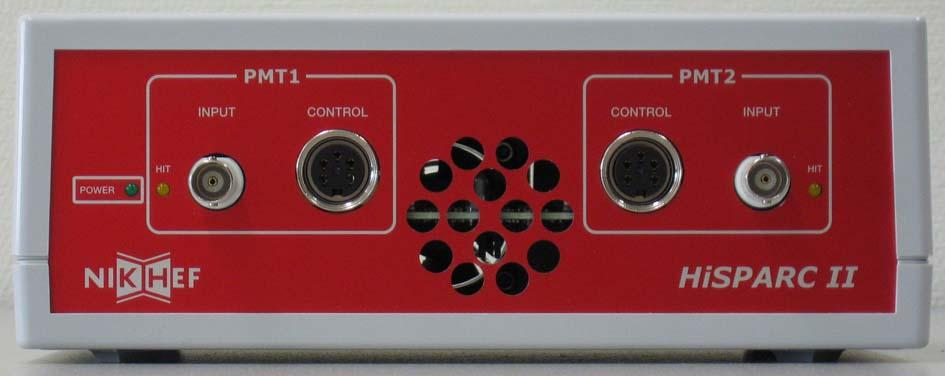
\includegraphics[scale=0.3]{kastje-voorkant}
    \caption{De voorkant van de \hisparc II Primary; van links naar
    rechts: groene LED voor de voedingsspanning, de gele LED geeft aan
    of er signalen binnenkomen, signaal- en voedingsaansluiting voor
    fotobuis-1. Midden: de inlaat voor de luchtkoeling. Rechts in
    omgekeerde volgorde: voedings- en signaalaansluiting fotobuis-2 en
    gele signaal LED.}
    \label{fig:kastje-voorkant}
\end{figure}

\begin{figure}
    \centering
    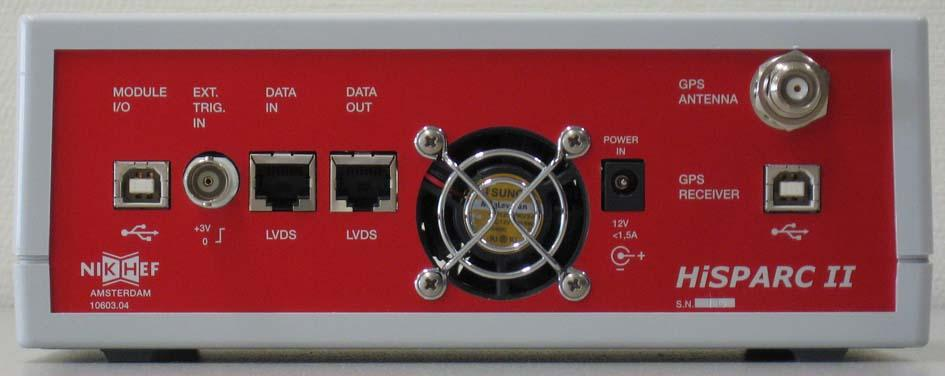
\includegraphics[scale=0.3]{primary-achterkant}
    \caption{De achterzijde van de \hisparc II Primary; van links naar
    rechts: USB aansluiting voor het versturen van de meetgegevens naar
    de pc, TTL aansluiting voor een externe trigger (alleen voor
    speciale doeleinden), twee UTP verbindingen (niet van toepassing),
    uitgang luchtkoeling, aansluiting voedingsadapter (12 Volt DC, 1.5
    A), GPS antenne aansluiting (rechtsboven) en USB verbinding voor het
    aanpassen van de GPS instellingen.}
    \label{fig:primary-achterkant}
\end{figure}

\subsection{Opstelling met vier skiboxen}

Om vier scintillatie detectoren uit te kunnen lezen, moet een tweede
\hisparc II unit aangesloten worden. Echter, deze unit – de Secondary –
\figref{fig:kastje-voorkant} bezit geen GPS maar is verder identiek aan de
Primary. Aan de achterzijde is dan ook geen aansluiting voor een
GPS-antenne aanwezig \figref{fig:primary-secondary-achterkant}.

\begin{figure}
    \centering
    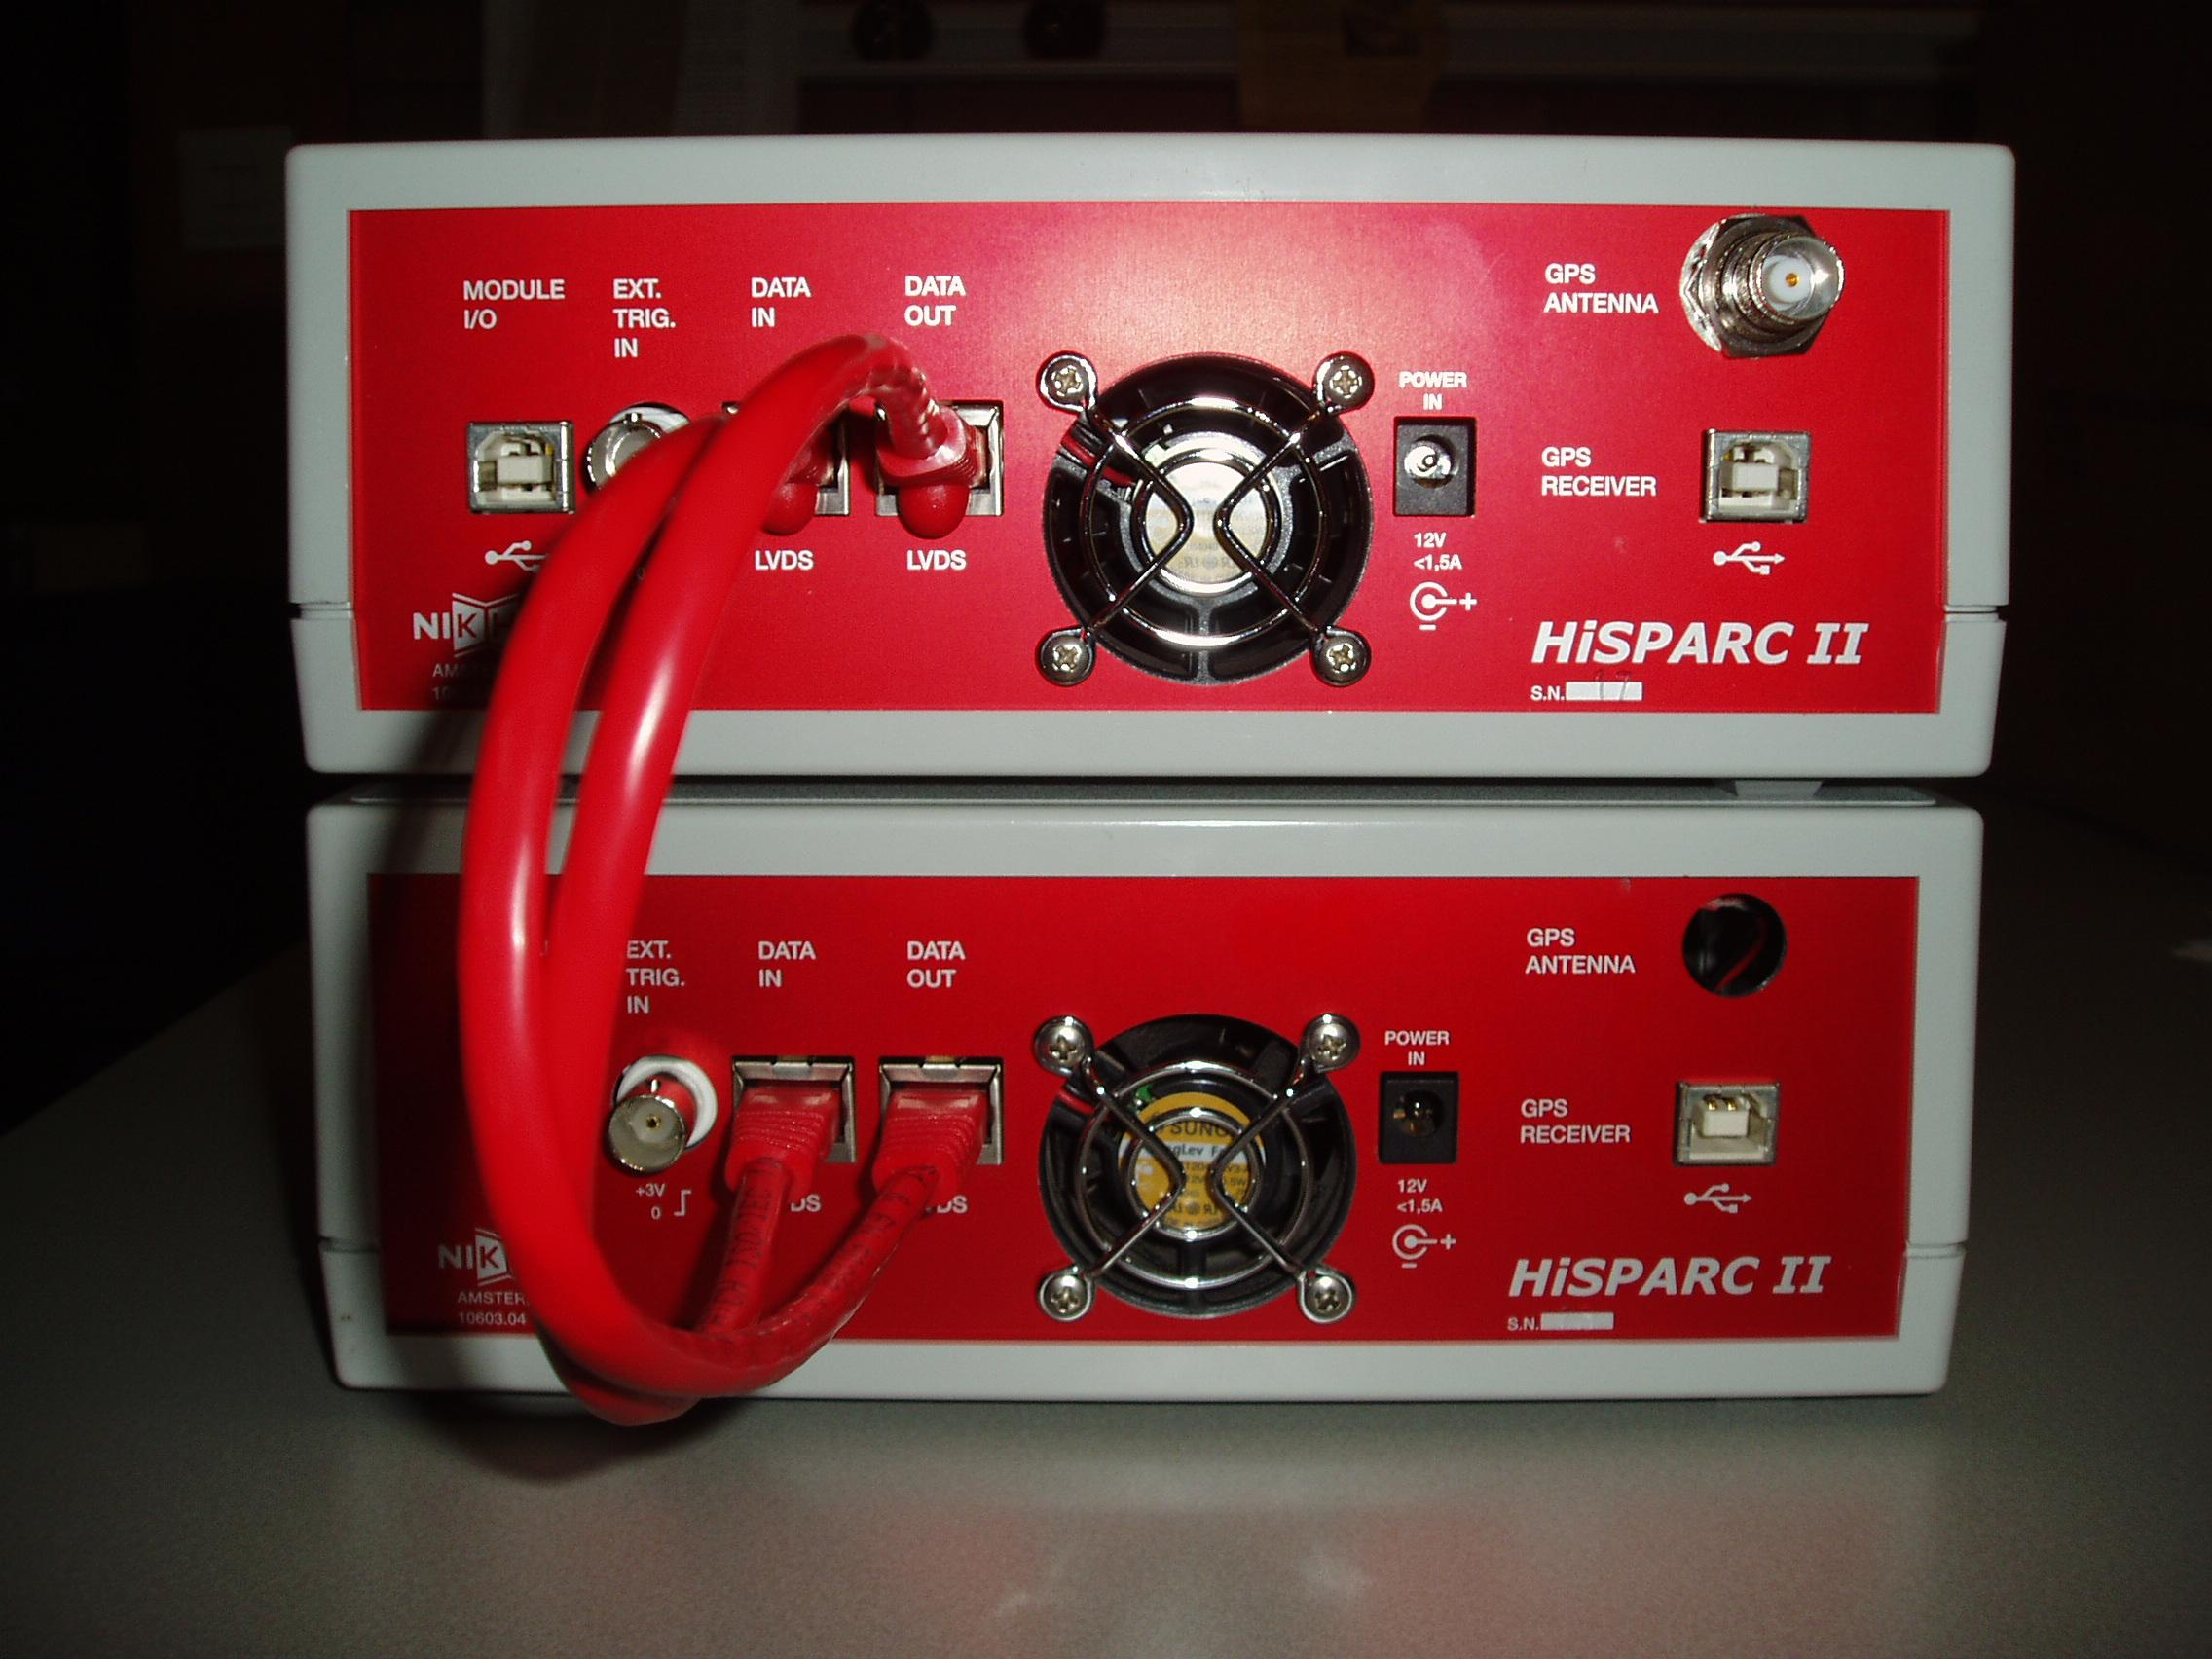
\includegraphics[scale=0.15]{primary-secondary-achterkant}
    \caption{Een snelle databus verzorgt de communicatie tussen \hisparc
    II Primary en Secondary; de verbinding bestaat uit twee kabels die ‘LVDS
    data in’ en ‘LVDS data out’ (kruislings) met elkaar verbinden.}
    \label{fig:primary-secondary-achterkant}
\end{figure}

De Secondary wordt via twee korte UTP kabels (kruislings, de lengte mag niet
veranderd worden!) verbonden met de Primary unit (Primary-Secondary
combinatie). Primary en Secondary versturen hun data dus over aparte USB
verbindingen (voor beide units is dit de linker connector aan de
achterzijde).

\end{document}
